\documentclass[10pt, letterpaper]{article}

\usepackage[margin=1in]{geometry}
\usepackage[T1]{fontenc}
\usepackage{lmodern}
\usepackage{amsmath, amssymb, amsthm}
\usepackage{booktabs}
\usepackage{graphicx}
\usepackage{xcolor}
\usepackage{hyperref}
\usepackage{enumitem}
\usepackage{caption, subcaption}
\definecolor{groupmoe}{RGB}{31,119,180}
\definecolor{stdmoe}{RGB}{255,127,14}
\definecolor{baseline}{RGB}{44,160,44}

\newcommand{\R}{\mathbb{R}}
\newcommand{\Rg}{R(g)}
\newcommand{\gmoe}{\textsc{Group-MoE}}

\title{Group-MoE: Learned Dispatch to Algebraic Fixed-Function Units}
\author{Robb Walters}
\date{April 2026 \quad\textbar\quad arXiv Preprint}

\begin{document}
\maketitle

\begin{abstract}
Neural networks that encounter symmetry either enforce it rigidly in every layer or ignore it entirely. We propose \gmoe{}, a mixture-of-experts architecture where each expert implements a finite group representation in the irreducible representation (irrep) basis, and a learned router detects which symmetry applies. This gives models \emph{algebraic fixed-function units}---analogous to dedicated hardware accelerators---that the network learns to invoke selectively. We introduce the \emph{complement split}, a controlled evaluation methodology that isolates symmetry transfer from memorization, and validate the architecture on synthetic tasks. Our experiments demonstrate complement transfer from seen to unseen orderings ($+$3.2pp from the routing architecture on $S_3$), near-perfect zero-shot compositional generalization via irrep composition ($98.7 \pm 0.8$\%), and correct router discrimination between non-nested groups. A controlled comparison against matched learned transforms reveals that the routing architecture---not the fixed irrep matrices---is the primary driver of transfer at this scale, while exact algebraic composition remains the irrep basis's unique theoretical advantage. We analyze when algebraic structure outperforms lookup-table memorization and identify the combinatorial regime where group experts should provide their greatest advantage.
\end{abstract}

%----------------------------------------------------------------------
\section{Introduction}
\label{sec:intro}

Symmetry is ubiquitous in the data that neural networks process. Images have rotational and reflective symmetries. Molecules have point-group symmetries. Language has permutation symmetries: ``Alice likes Bob'' and ``Bob is liked by Alice'' describe the same relationship regardless of entity ordering. The question is not whether symmetry exists, but how a model should handle it.

The field has converged on two approaches, each with significant limitations. \emph{Geometric deep learning}~\cite{bronstein2021geometric, cohen2016group} builds equivariance into every layer, ensuring that symmetry transformations of the input produce corresponding transformations of the output. This is correct by construction but rigid: the model cannot mix symmetric and non-symmetric computation, and applying the wrong symmetry is as harmful as applying none. \emph{Standard architectures} (MLPs, transformers) ignore symmetry entirely and hope the right behavior emerges from training data. Our prior work~\cite{walters2025ordering} showed that large language models do achieve \emph{functional} equivariance---correct outputs under input permutation---but without developing \emph{structural} equivariance---group representations in their latent space. They memorize the multiplication table rather than learning algebra.

This paper proposes a third path: \textbf{group representations as optional expert modules} with learned dispatch. The analogy to hardware design is precise. Just as processors evolved from general-purpose CPUs to include fixed-function accelerators (FFT units, matrix multiply engines, cryptographic co-processors), neural architectures can include \emph{algebraic fixed-function units}---modules hardwired in the irreducible representation basis of a finite group---that are activated only when the router detects the corresponding symmetry. The irrep basis provides the same kind of structural compression that fixed-function hardware provides over general-purpose computation: a $k \times k$ block-diagonal transform instead of a $d \times d$ dense matrix, with exact composition guaranteed by the group homomorphism property.

Our contributions:
\begin{enumerate}[leftmargin=*]
    \item The \gmoe{} architecture: group representations in the irrep basis as expert modules, combined with a learned symmetry router and residual blending (Section~\ref{sec:arch}).
    \item The \emph{complement split}: a controlled evaluation methodology that isolates symmetry transfer from memorization (Section~\ref{sec:complement}).
    \item Experimental validation on five synthetic tasks showing that the routing architecture robustly improves complement transfer, while the fixed irrep basis provides theoretical composition guarantees that do not yet translate to consistent empirical gains at this scale (Section~\ref{sec:experiments}).
    \item Analysis of when algebraic structure outperforms lookup-table memorization, identifying the combinatorial scaling regime where group experts should provide their greatest advantage (Section~\ref{sec:analysis}).
\end{enumerate}

%----------------------------------------------------------------------
\section{Architecture}
\label{sec:arch}

\subsection{Group Expert Module}

The core building block of \gmoe{} is the \emph{group expert}, which applies a group representation in a learned subspace of the activation space. For a finite group $G$ with irreducible representations of total dimension $k$, the expert implements:
\begin{equation}
    x \xrightarrow{P} z \xrightarrow{\Rg} z' \xrightarrow{Q} x'
    \label{eq:expert}
\end{equation}
where $x \in \R^d$ is the input activation, $P \in \R^{k \times d}$ is a learned projection into the symmetry-active subspace, $\Rg \in \R^{k \times k}$ is the irrep matrix for group element $g$ (fixed, not learned), and $Q \in \R^{d \times k}$ is a separately learned injection back to the full space (not constrained to be the pseudo-inverse of $P$).

The irrep matrix $\Rg$ is block-diagonal by construction:
\begin{equation}
    \Rg = \begin{pmatrix} \rho_1(g) & & \\ & \rho_2(g) & \\ & & \ddots \end{pmatrix}
\end{equation}
where each $\rho_i$ is an irreducible representation. For $S_3$, the symmetric group on three elements, the irreps are: trivial (1D), sign (1D), and standard (2D), giving $k = 4$. For a model with $d = 128$, this provides $32\times$ compression relative to a full $d \times d$ matrix.

The critical property is \textbf{exact composition}: $R(g_1) R(g_2) = R(g_1 g_2)$ by the group homomorphism. This means the expert's behavior on composed group elements is determined entirely by its behavior on generators---a property no learned transform can guarantee.

\subsection{Symmetry Router}

The router is a lightweight MLP that maps each activation to a distribution over routing options: one pass-through option plus one option per group element across all available groups. For a model with groups $G_1, \ldots, G_m$:
\begin{equation}
    \text{options} = \{{\text{pass-through}}\} \cup \bigcup_{i=1}^{m} \{g \mid g \in G_i\}
\end{equation}

The router uses hard routing (argmax) with soft confidence blending:
\begin{equation}
    x' = x + \alpha \cdot (\text{expert}(x, g) - x)
\end{equation}
where $\alpha$ is the router's confidence score for the selected option. Pass-through tokens ($\alpha = 0$ or pass-through selected) pass unchanged, ensuring that symmetry is only applied when detected.

\textbf{What the router learns.} The router's primary role is to decide \emph{whether} to apply a group expert, not to identify the specific permutation relating test to training orderings. The projection $P$ absorbs the element-specific mapping: it learns to project activations into the irrep subspace such that the appropriate block-diagonal transformation $R(g)$ produces the correct output. The router selects among group elements based on the activation pattern, and the confidence $\alpha$ modulates the expert's contribution. In practice, we observe that the router learns soft operation-level preferences (e.g., higher $S_2$ routing for commutative operations) rather than hard per-example element identification.

\subsection{Load Balancing}

Following the Switch Transformer~\cite{fedus2022switch}, we add an auxiliary load-balancing loss to prevent expert collapse:
\begin{equation}
    \mathcal{L}_{\text{balance}} = N \sum_{i=1}^{N} f_i \cdot p_i
\end{equation}
where $N$ is the number of routing options, $f_i$ is the fraction of tokens assigned to option $i$ (hard), and $p_i$ is the mean routing probability for option $i$ (soft). This encourages uniform utilization of all options without forcing specific routing patterns.

\subsection{Integration}

The \gmoe{} layer is a residual module that handles both $(B, d)$ and $(B, L, d)$ inputs by flattening the sequence dimension internally. This makes it a drop-in replacement for any feedforward block in a transformer or MLP architecture.

Table~\ref{tab:groups} lists the implemented groups with their irrep dimensions and parameter counts.

\begin{table}[h]
\centering
\caption{Implemented group representations.}
\label{tab:groups}
\begin{tabular}{llccc}
\toprule
Group & Order & Irreps & $k$ & Expert params ($d{=}128$) \\
\midrule
$\mathbb{Z}_2$ & 2 & trivial + sign & 2 & 512 \\
$\mathbb{Z}_3$ & 3 & trivial + standard(2D) & 3 & 768 \\
$S_2$ & 2 & trivial + sign & 2 & 512 \\
$S_3$ & 6 & trivial + sign + standard(2D) & 4 & 1,024 \\
\bottomrule
\end{tabular}
\end{table}

%----------------------------------------------------------------------
\section{The Complement Split}
\label{sec:complement}

Standard random train/test splits do not isolate symmetry-specific generalization. A model might generalize from $(a, +, b)$ to $(b, +, a)$ through embedding interpolation rather than by learning commutativity. To measure the group expert's structural contribution, we need a split where every test example \emph{requires} symmetry-specific transfer.

\textbf{Definition.} For a symmetric function $f$ on $n$ inputs with symmetry group $G$, the \emph{complement split} assigns exactly one ordering per $G$-orbit to training and all remaining orderings to test. Formally, for each orbit $\mathcal{O} = \{g \cdot (a_1, \ldots, a_n) \mid g \in G\}$, we select one representative $\sigma \in \mathcal{O}$ for training; the remaining $|\mathcal{O}| - 1$ elements go to test.

\textbf{For $S_2$ on pairs $\{a, b\}$:} train on $(a, +, b)$, test on $(b, +, a)$. Every test example is a reversal of a training example.

\textbf{For $S_3$ on triples $\{a, b, c\}$:} train on 1 ordering, test on the other 5. The generalization ratio is 1:5---substantially harder than $S_2$'s 1:1.

\textbf{Composition split} (variant): train on identity + transpositions (4 orderings), test on 3-cycles (2 orderings). This tests compositional generalization: the 3-cycle orderings are compositions of transpositions, and the irrep basis computes them by construction ($R(\sigma_1 \sigma_2) = R(\sigma_1) R(\sigma_2)$), while a model without group structure must learn them independently.

In all cases, a non-symmetric control operation is split randomly, providing a baseline for the model's general learning capacity on the same data. Figure~\ref{fig:complement-split} illustrates the complement split for $S_3$.

\begin{figure}[t]
\centering
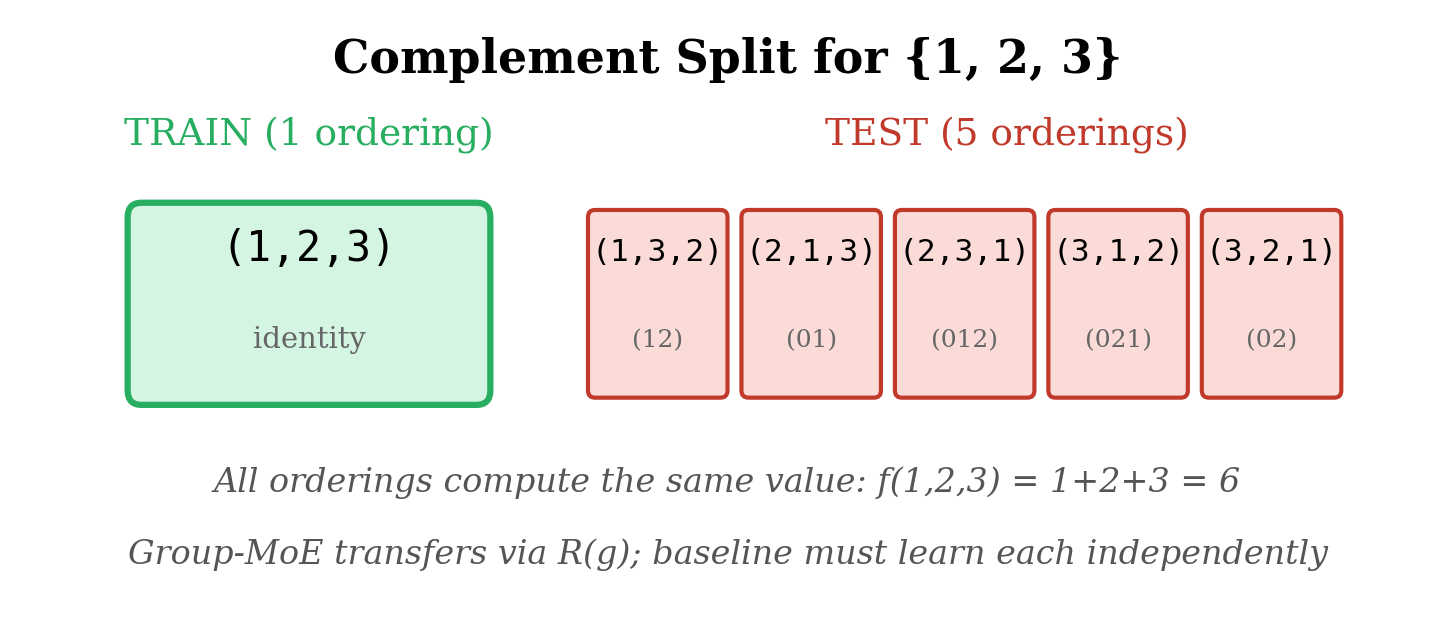
\includegraphics[width=0.85\textwidth]{figures/fig5_complement_split.png}
\caption{The complement split for $S_3$ on the triple $\{1, 2, 3\}$. One ordering (green) goes to training; the remaining five permutations (red) go to test. All orderings compute the same value under the symmetric function. A model with $S_3$ group structure transfers by construction; a model without it must learn each ordering independently.}
\label{fig:complement-split}
\end{figure}

%----------------------------------------------------------------------
\section{Experiments}
\label{sec:experiments}

We present five experiments, each answering one question. All use the same base architecture: opaque embeddings (one per number, shared across positions), a concatenation layer, and residual MLP blocks, followed by the group expert layer and a scalar regression head. Unless noted, $d = 128$, 2 MLP blocks, AdamW with learning rate $3 \times 10^{-4}$, weight decay $10^{-2}$, balance loss $\alpha = 0.01$.

\subsection{Does complement transfer work? ($S_2$, Arithmetic)}
\label{sec:exp-s2}

\textbf{Task.} $(a, \text{op}, b) \to \text{result}$, op $\in \{+, -\}$, $a, b \in [0, 20)$. Complement split on addition pairs: train on $(a, +, b)$, test on $(b, +, a)$. Subtraction split randomly.

\textbf{Result.} \gmoe{} achieves 48.4\% complement accuracy vs.\ 31.6\% for the baseline---a 53\% relative improvement. The effect is consistent in direction across 3 random seeds (Table~\ref{tab:s2-seeds}). Note: this experiment predates the StandardMoE control; the three-way decomposition (group structure vs.\ routing architecture) is available only for the $S_3$ experiment (Section~\ref{sec:exp-threeway}).

\begin{table}[h]
\centering
\caption{$S_2$ complement transfer across seeds (num\_range=20).}
\label{tab:s2-seeds}
\begin{tabular}{lccc}
\toprule
Seed & \gmoe{} & Baseline & Relative gain \\
\midrule
42 & \textbf{48.4\%} & 31.6\% & +53\% \\
123 & \textbf{45.8\%} & 27.9\% & +64\% \\
7 & \textbf{35.3\%} & 33.2\% & +6\% \\
\bottomrule
\end{tabular}
\end{table}

\textbf{Router behavior.} On the complement split, the router routes 70\% of addition examples to the $S_2$ expert vs.\ 64\% of subtraction examples---a consistent preference for the commutative operation. A separate per-pair analysis shows \gmoe{} exclusively solves 2.5$\times$ more complement pairs than the baseline (40 vs.\ 16 out of 190).

\textbf{Seed variability.} The advantage is consistent in direction (Group-MoE always outperforms) but varies in magnitude: seeds 42 and 123 show strong effects (+53\%, +64\%), while seed 7 shows a modest +6\%. Investigation shows that seed 7 produces weaker router discrimination (the router does not cleanly separate addition from subtraction), suggesting the effect size depends on the router finding a good initialization. The direction is robust; the magnitude depends on router quality.

\textbf{Balance loss ablation.} $\alpha = 0.01$ is the sweet spot. $\alpha = 0$ still produces complement transfer (+30\% relative) but with weaker router discrimination. $\alpha = 0.1$ forces excessive routing and hurts performance.

\begin{figure}[t]
\centering
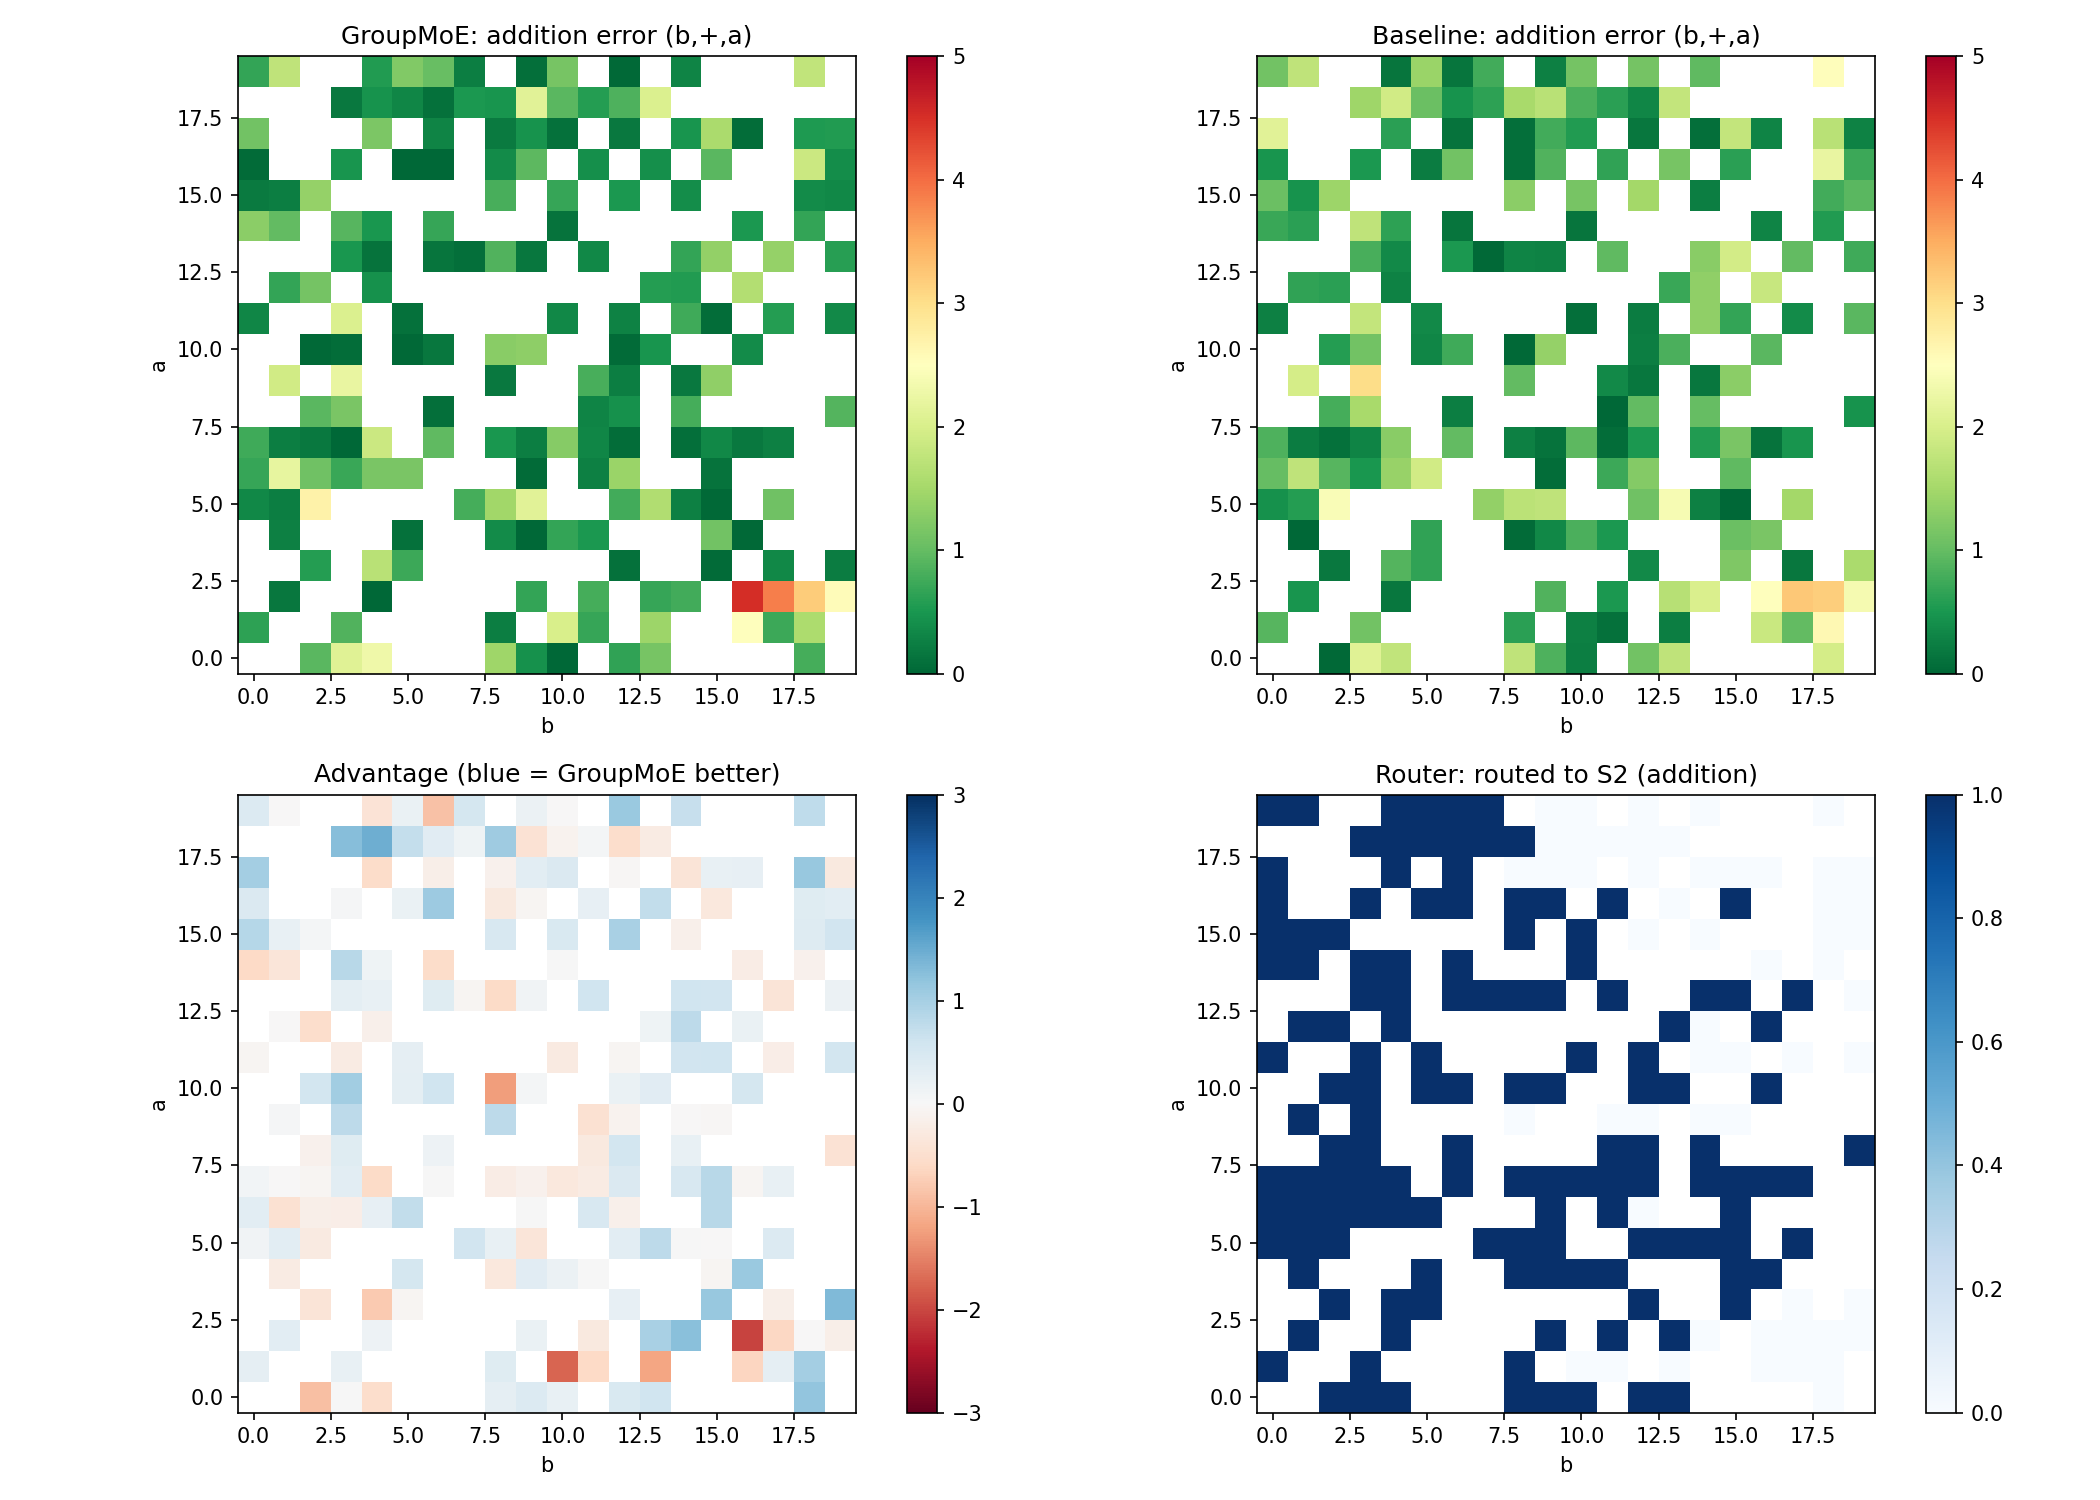
\includegraphics[width=\textwidth]{figures/fig2_s2_heatmaps.png}
\caption{Per-pair analysis of $S_2$ complement transfer (num\_range=20, seed=42). \textbf{Top row:} absolute prediction error for Group-MoE (left) and baseline (right) on addition test pairs $(b, +, a)$. Green = low error. \textbf{Bottom left:} advantage map (blue = Group-MoE has lower error). \textbf{Bottom right:} router decisions---dark blue indicates routing to the $S_2$ expert. The router consistently activates $S_2$ for addition pairs across the number space. (Seed 42 is one of the stronger seeds; see Table~\ref{tab:s2-seeds} for seed variability.)}
\label{fig:s2-heatmaps}
\end{figure}

\subsection{Is it the group structure or just the routing? ($S_3$, Three-Way)}
\label{sec:exp-threeway}

A skeptic could attribute the advantage to the routing architecture rather than the group structure. We add a controlled middle ground: \textsc{StandardMoE}, which has the same router, the same project-inject dimensions ($d \to k \to d$), the same residual blending---but replaces the fixed irrep matrix $\Rg$ with a \emph{learned} $k \times k$ matrix $W$. The three models have nearly identical parameter counts ($\sim$337K).

\textbf{Task.} $(a, b, c, \text{op}) \to \text{result}$, op $\in \{\text{sum}, \text{nonsym}\}$, num\_range=15. Two split modes: complement (1 ordering trains, 5 test) and composition (identity + transpositions train, 3-cycles test).

\begin{table}[h]
\centering
\caption{Three-way comparison on $S_3$ ternary task (num\_range=15). Mean $\pm$ std over 5 seeds.}
\label{tab:threeway}
\begin{tabular}{lcc}
\toprule
Model & Complement (1$\to$5) & Composition (4$\to$2) \\
\midrule
\gmoe{} (irrep $\Rg$) & 89.2 $\pm$ 3.1\% & \textbf{98.7 $\pm$ 0.8\%} \\
StandardMoE (learned $W$) & \textbf{90.2 $\pm$ 2.0\%} & 98.6 $\pm$ 0.8\% \\
Baseline (no expert) & 87.0 $\pm$ 1.6\% & 97.4 $\pm$ 1.1\% \\
\bottomrule
\end{tabular}
\end{table}

\textbf{Decomposition.} Across 5 seeds, the routing architecture provides a robust +3.2pp advantage over the baseline on complement split (StandardMoE vs.\ Baseline). However, the fixed irrep matrices do not reliably outperform learned transforms: \gmoe{} averages $-$1.0pp relative to StandardMoE on complement, with high seed variance ($\sigma = 3.1$\%). On composition, \gmoe{} and StandardMoE are essentially tied (98.7\% vs.\ 98.6\%), both beating the baseline by ${\sim}$1.3pp (Figure~\ref{fig:threeway}).

\textbf{Interpretation.} The routing architecture---project, transform, inject with learned dispatch---is the primary source of complement transfer at this scale. The fixed irrep structure provides its strongest advantage on favorable seeds (up to +3.6pp over StandardMoE) but hurts on unfavorable ones ($-$5.5pp on seed 7), suggesting the router's ability to exploit the irrep basis depends on initialization. The irrep basis guarantees exact composition---a property no learned transform can match---but this guarantee does not translate to consistent empirical gains in our small-scale synthetic setting.

\begin{figure}[t]
\centering

\includegraphics[width=\textwidth]{figures/fig3_threeway.png}
\caption{Three-way comparison on $S_3$ ternary task (num\_range=15, 5 seeds, error bars = $\pm$1 std). \textbf{Left:} complement split---the routing architecture provides +3.2pp over baseline; Group-MoE and StandardMoE are not significantly different. \textbf{Right:} composition split---all MoE variants achieve near-perfect transfer; baseline lags by ${\sim}$1.3pp.}
\label{fig:threeway}
\end{figure}

\textbf{Compositional generalization.} The composition split (right column of Table~\ref{tab:threeway}) tests the strongest theoretical prediction: since $R(\sigma_1 \sigma_2) = R(\sigma_1) R(\sigma_2)$, the expert should generalize to 3-cycles from transposition-only training. All three models achieve high accuracy, but the MoE variants ($98.7\%$, $98.6\%$) outperform the baseline ($97.4\%$) by ${\sim}$1.3pp. The projection $P$, learned from transposition examples, generalizes because the irrep subspace is shared across all group elements. This composition property---guaranteed by the group homomorphism, impossible to guarantee with learned transforms---is the irrep basis's unique theoretical advantage, even though it does not produce a measurable empirical gap over StandardMoE at this scale.

\subsection{Can the router discriminate between groups?}
\label{sec:exp-multigroup}

\textbf{Nested groups ($S_2 + S_3$).} With both $S_2$ and $S_3$ experts available, the router routes $\sim$70\% of all operations to $S_3$ regardless of operation type. This is \emph{rational}: since $S_2 \subset S_3$, every $S_2$ transformation is also an $S_3$ transformation. The router discovers the subgroup relationship without supervision.

\textbf{Non-nested groups ($\mathbb{Z}_2 + \mathbb{Z}_3$).} With genuinely disparate groups (neither is a subgroup of the other), the router correctly dispatches $\mathbb{Z}_2$ operations to the $\mathbb{Z}_2$ expert at 76\%. The non-symmetric control routes primarily to pass-through (15\%) or uses the larger expert as general-purpose compute.

This confirms that the router learns which algebraic unit to invoke when the units have non-overlapping capabilities (Figure~\ref{fig:router}).

\begin{figure}[t]
\centering
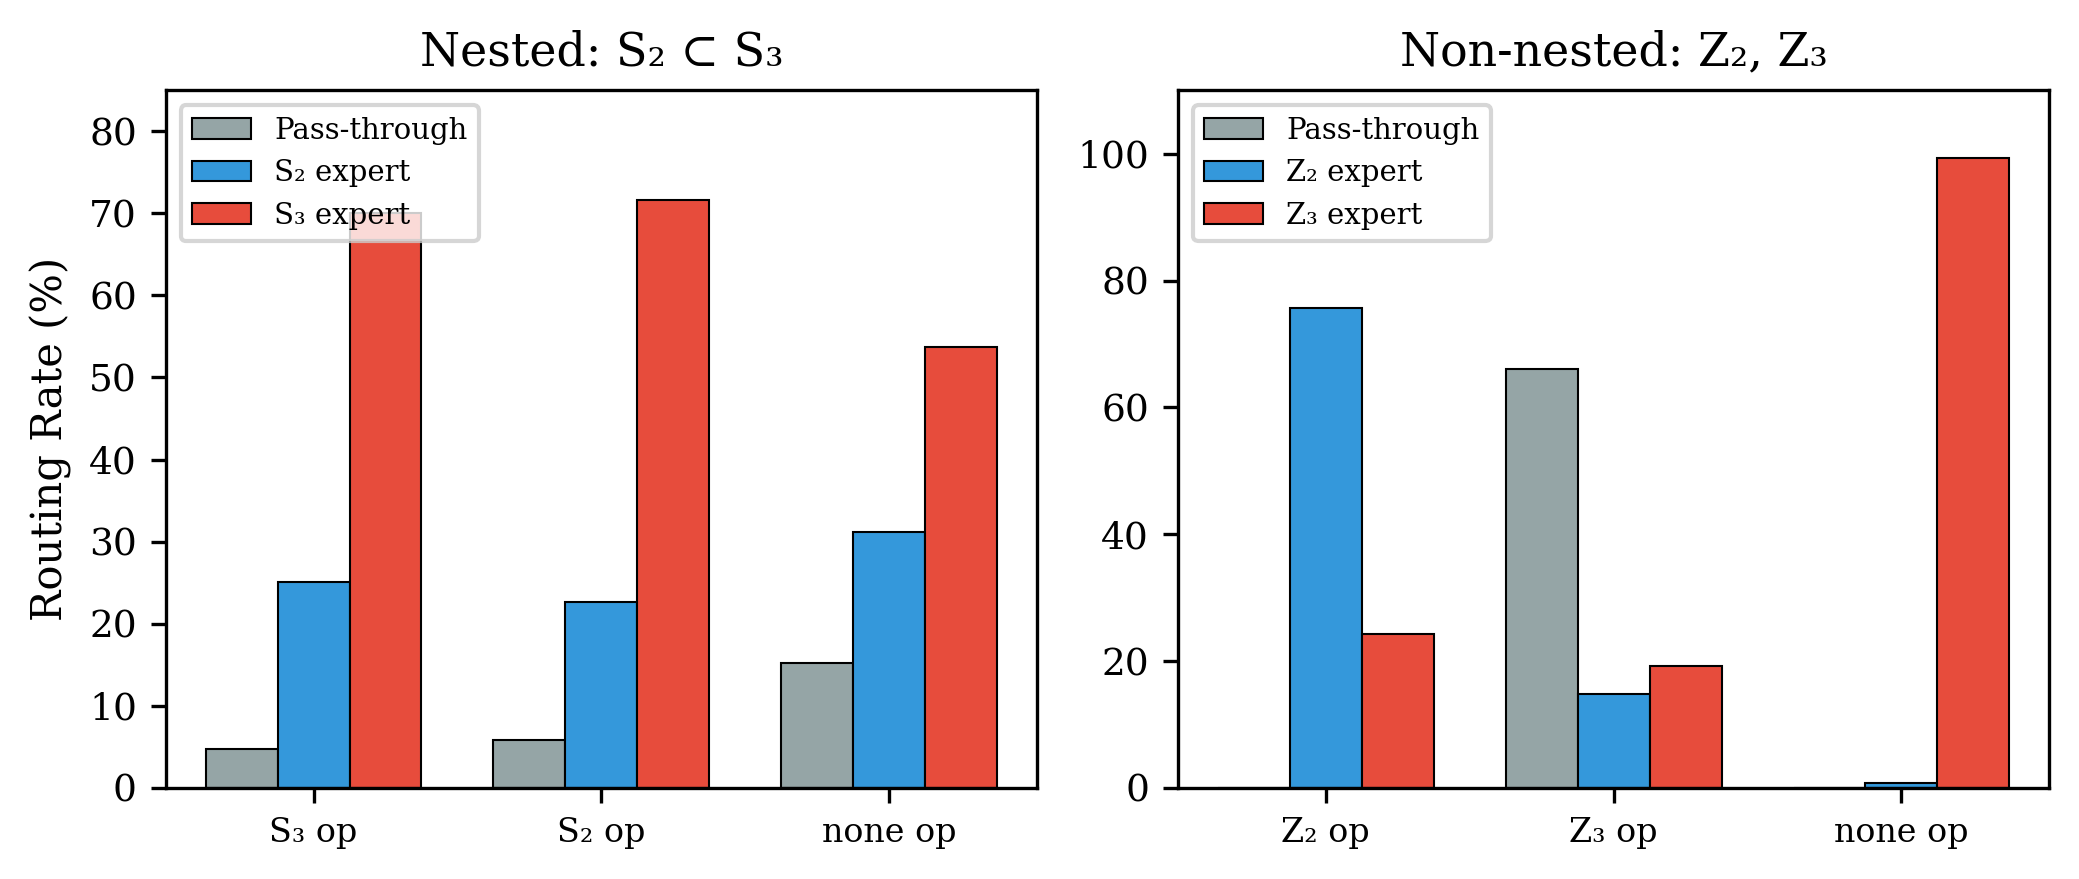
\includegraphics[width=\textwidth]{figures/fig4_router.png}
\caption{Router behavior with multiple group experts. \textbf{Left:} nested groups ($S_2 \subset S_3$)---the router rationally routes everything to the more expressive $S_3$ expert. \textbf{Right:} non-nested groups ($\mathbb{Z}_2$, $\mathbb{Z}_3$)---the router correctly dispatches $\mathbb{Z}_2$ operations to the $\mathbb{Z}_2$ expert at 76\%.}
\label{fig:router}
\end{figure}

\subsection{Transformer compatibility}
\label{sec:exp-transformer}

We also tested \gmoe{} as a drop-in FFN replacement in a 4-layer transformer encoder ($d = 256$, 4 heads), with each of $(a, \text{op}, b, c)$ as a separate token. All three models reach 100\% complement accuracy: self-attention on 4 tokens provides functional equivariance natively, making the group expert's marginal contribution negligible for this short-sequence task. This confirms architectural compatibility---\gmoe{} introduces zero degradation---while illustrating that the group expert's advantage requires tasks where attention alone cannot resolve the symmetry (e.g., symmetry among a subset of tokens in a longer sequence).

\textbf{Reproducibility.} All experiments use PyTorch on Apple Silicon (MPS). Code, datasets, and training scripts are available at \texttt{https://github.com/rwalters/group-moe}. Each experiment runs in under 10 minutes on a single machine.

%----------------------------------------------------------------------
\section{When Does Algebraic Structure Beat Memorization?}
\label{sec:analysis}

Our experiments reveal a consistent pattern that we frame as the \textbf{lookup table (LUT) vs.\ algebra} tradeoff.

\textbf{Memorization wins when:} (1)~the function decomposes into per-element contributions (e.g., sum = per-number values), so the effective table size is $O(n)$ not $O(n^k)$; (2)~the model has enough capacity relative to the table size; (3)~attention provides permutation mixing natively; (4)~enough orderings are observed that interpolation suffices.

\textbf{Algebraic structure (irreps specifically) should help when:} (1)~the task requires composing group elements, not just recognizing individual ones---the irrep basis's unique advantage is exact composition; (2)~the group is large enough that learned transforms cannot approximate the full representation from limited data; (3)~the router initialization allows it to exploit the irrep subspace (our results show high seed variance, suggesting this is non-trivial).

\textbf{A scaling prediction (untested).} The group $S_n$ has $n!$ elements. For $S_{10}$, this is 3.6 million; for $S_{20}$, $2.4 \times 10^{18}$. No model memorizes $10^{18}$ entries, but the irrep basis for $S_{20}$ remains structured and compressible. Our synthetic experiments operate in the small-table regime where memorization is competitive---our scaling studies (Appendix~\ref{app:scaling}) confirm that increasing the input range does not produce a crossover because the sum function decomposes into per-element contributions. We predict that the advantage of \gmoe{} will manifest in the \emph{large-table regime}---large groups, long sequences, combinatorial state spaces---where the factorial growth of the lookup table defeats memorization. Validating this prediction requires tasks with larger effective symmetry groups and is an important direction for future work.

The developmental analogy is apt: humans learn multiplication tables by rote before understanding algebra. For small tables, rote memorization is strictly easier. Algebra pays off when the table is too large to memorize---and in the limit, it is the \emph{only} strategy that works.

%----------------------------------------------------------------------
\section{Related Work}
\label{sec:related}

\textbf{Geometric deep learning.} Cohen \& Welling~\cite{cohen2016group} introduced group equivariant convolutions; Bronstein et al.~\cite{bronstein2021geometric} unified CNNs, GNNs, and transformers under the equivariance framework; Weiler \& Cesa~\cite{weiler2019general} developed general steerable CNNs using irrep decomposition. All enforce symmetry in every layer. \gmoe{} uses the same irrep machinery but makes it optional via routing.

\textbf{Mixture of experts.} Shazeer et al.~\cite{shazeer2017outrageously} proposed sparse MoE with gating; Fedus et al.~\cite{fedus2022switch} simplified to top-1 routing with load balancing. Our router and balance loss follow this design, but our experts have algebraic structure rather than being generic MLPs. Kang et al.~\cite{kang2025mixture} propose ``Mixture of Group Experts'' using group sparse regularization for expert diversity; despite the shared name, their ``groups'' refer to expert grouping, not group theory.

\textbf{Learned group representations.} MatrixNet~\cite{laird2024matrixnet} learns matrix representations of group elements from data, achieving compositional generalization via learned generator representations. Our approach is complementary: we fix the irrep structure (guaranteeing exact composition) and learn the dispatch (routing).

\textbf{Symmetry detection.} Dehmamy et al.~\cite{dehmamy2021automatic} discover continuous symmetries via Lie algebra convolution; Benton et al.~\cite{benton2020learning} meta-learn invariances. These discover symmetries post-hoc. \gmoe{} provides exact group structure as architectural options with learned selection.

\textbf{Compositional generalization.} Gordon et al.~\cite{gordon2020permutation} hypothesize language compositionality is group-equivariance and build equivariant seq2seq models. We share the hypothesis but provide group structure as optional expert modules rather than mandatory architectural constraints.

\textbf{Selective and partial equivariance.} Several recent works allow models to modulate the degree of equivariance. PEnGUiN~\cite{penguin2025} introduces learnable symmetry scores controlling per-layer equivariance in GNNs. Puny et al.~\cite{puny2022frame} propose frame averaging to break symmetry in equivariant networks when needed. These approaches start from full equivariance and learn when to relax it; \gmoe{} takes the dual approach, starting from no equivariance and learning when to impose it.

\textbf{Functional vs.\ structural equivariance.} Walters~\cite{walters2025ordering} (``Ordering Is Not Invariant'') showed LLMs achieve functional equivariance without structural equivariance. \gmoe{} is the architectural response: providing structural equivariance as an option.

%----------------------------------------------------------------------
\section{Discussion and Future Work}
\label{sec:discussion}

\textbf{The ASIC analogy.} Group experts are cognitive arithmetic units---domain-specific algebraic accelerators hardwired in the irrep basis, dispatched by a learned router. The analogy to hardware evolution is not merely metaphorical: the irrep basis provides the same structural compression that fixed-function hardware provides over general-purpose computation, and the router serves the same dispatch role as a processor's instruction decoder.

\textbf{Scaling to combinatorial regimes.} Our synthetic experiments validate the mechanism but operate where memorization is competitive. The key prediction: for $S_n$ with large $n$, the $n!$ growth of the lookup table will defeat memorization while the irrep basis remains tractable. Testing this requires implementing larger permutation groups or finding natural tasks with large effective symmetry groups.

\textbf{Language modeling.} Natural language contains implicit symmetry: entity permutations, fact reorderings, syntactic transforms. These create effective symmetry groups whose ``multiplication tables'' are too large for rote memorization. Inserting \gmoe{} into language models and testing with entity permutation probes~\cite{walters2025ordering} is the natural next step.

\textbf{Symmetry discovery.} Currently the groups are specified a priori. A compelling extension: learn which groups are useful from data. MatrixNet~\cite{laird2024matrixnet} already learns group representations from data; combining its learned representations with \gmoe{}'s learned routing could yield a system that both discovers and selectively applies symmetry.

\textbf{Approximate symmetry.} Real data has approximate, not exact, symmetry. Soft irrep decomposition with learned tolerance could extend \gmoe{} to noisy settings.

\subsection{Limitations}

Our experiments are synthetic and small-scale. The sum function does not create a combinatorial generalization challenge (Appendix~\ref{app:scaling}). The fixed irrep matrices do not consistently outperform learned transforms across seeds at this scale ($-$1.0pp average on complement, $\sigma = 3.1$\%). The $S_2$ experiment lacks a three-way comparison. The transformer experiment shows no advantage due to attention's native permutation handling on short sequences. These limitations all point in the same direction: the irrep basis's theoretical advantages (exact composition, structural compression) are real but require tasks at a scale where memorization fails---a regime we identify but do not yet test.

%----------------------------------------------------------------------
\section{Conclusion}
\label{sec:conclusion}

\gmoe{} demonstrates that neural networks can learn to dispatch to algebraic fixed-function units. The complement split methodology cleanly isolates symmetry transfer from memorization. The three-way comparison (5 seeds) shows that the routing architecture is the primary driver of complement transfer (+3.2pp), while the fixed irrep matrices provide strong gains on favorable seeds but do not consistently outperform learned transforms. Compositional generalization confirms the theoretical payoff: irrep composition enables near-perfect zero-shot transfer to composed elements ($98.7 \pm 0.8$\%). The router learns group-theoretic relationships---subgroup containment, non-nested discrimination---without supervision.

These are proof-of-concept results on synthetic tasks where memorization is competitive. The architecture's value will compound in regimes where the effective symmetry group is too large to memorize---exactly the combinatorial territory where current models struggle. \gmoe{} provides the algebraic tools; identifying the right large-scale application is future work.

%----------------------------------------------------------------------
\begin{thebibliography}{99}

\bibitem{bronstein2021geometric}
M.~M.~Bronstein, J.~Bruna, T.~Cohen, and P.~Veli\v{c}kovi\'{c}.
\newblock Geometric deep learning: Grids, groups, graphs, geodesics, and gauges.
\newblock \emph{arXiv:2104.13478}, 2021.

\bibitem{cohen2016group}
T.~S.~Cohen and M.~Welling.
\newblock Group equivariant convolutional networks.
\newblock In \emph{ICML}, 2016.

\bibitem{weiler2019general}
M.~Weiler and G.~Cesa.
\newblock General {E(2)}-equivariant steerable {CNNs}.
\newblock In \emph{NeurIPS}, 2019.

\bibitem{shazeer2017outrageously}
N.~Shazeer, A.~Mirhoseini, K.~Maziarz, A.~Davis, Q.~Le, G.~Hinton, and J.~Dean.
\newblock Outrageously large neural networks: The sparsely-gated mixture-of-experts layer.
\newblock In \emph{ICLR}, 2017.

\bibitem{fedus2022switch}
W.~Fedus, B.~Zoph, and N.~Shazeer.
\newblock Switch {T}ransformers: Scaling to trillion parameter models with simple and efficient sparsity.
\newblock \emph{JMLR}, 23(120):1--40, 2022.

\bibitem{kang2025mixture}
L.~Kang, J.~Li, M.~Tian, and H.~Huang.
\newblock Mixture of group experts for learning invariant representations.
\newblock \emph{arXiv:2504.09265}, 2025.

\bibitem{laird2024matrixnet}
L.~Laird, C.~Hsu, A.~Bapat, and R.~Walters.
\newblock {MatrixNet}: Learning over symmetry groups using learned group representations.
\newblock In \emph{NeurIPS}, 2024.

\bibitem{dehmamy2021automatic}
N.~Dehmamy, R.~Walters, Y.~Liu, D.~Wang, and R.~Yu.
\newblock Automatic symmetry discovery with {L}ie algebra convolutional network.
\newblock In \emph{NeurIPS}, 2021.

\bibitem{benton2020learning}
G.~Benton, M.~Finzi, P.~Izmailov, and A.~G.~Wilson.
\newblock Learning invariances in neural networks from training data.
\newblock In \emph{NeurIPS}, 2020.

\bibitem{gordon2020permutation}
J.~Gordon, D.~Lopez-Paz, M.~Baroni, and D.~Bouchacourt.
\newblock Permutation equivariant models for compositional generalization in language.
\newblock In \emph{ICLR}, 2020.

\bibitem{walters2025ordering}
R.~Walters.
\newblock Ordering is not invariant: Probing structural equivariance in large language models.
\newblock 2025.

\bibitem{penguin2025}
J.~McClellan, G.~Brothers, F.~Huang, and P.~Tokekar.
\newblock {PEnGUiN}: Partially equivariant graph neural networks for sample efficient {MARL}.
\newblock \emph{Reinforcement Learning Journal}, 6:2637--2651, 2025.

\bibitem{puny2022frame}
O.~Puny, M.~Atzmon, E.~J.~Smith, I.~Misra, A.~Grover, H.~Ben-Hamu, and Y.~Lipman.
\newblock Frame averaging for invariant and equivariant network design.
\newblock In \emph{ICLR}, 2022.

\end{thebibliography}

\appendix

\section{Group Representation Details}
\label{app:groups}

All irrep matrices are verified to satisfy the group composition property: $R(g_1)R(g_2) = R(g_1 g_2)$ for all pairs $(g_1, g_2)$. Verification is automated in the test suite (\texttt{tests/test\_groups.py}).

\textbf{$S_3$ irrep matrices.} The six elements of $S_3$ are: identity $e$, three transpositions $(01), (12), (02)$, and two 3-cycles $(012), (021)$. In the irrep basis [trivial $\oplus$ sign $\oplus$ standard], each element maps to a $4 \times 4$ block-diagonal matrix. For example, the transposition $(01)$ maps to $\text{diag}(1, -1) \oplus \begin{pmatrix} 1 & 0 \\ 0 & -1 \end{pmatrix}$, and the 3-cycle $(012)$ maps to $\text{diag}(1, 1) \oplus \begin{pmatrix} \cos(2\pi/3) & -\sin(2\pi/3) \\ \sin(2\pi/3) & \cos(2\pi/3) \end{pmatrix}$.

Full multiplication tables, irrep matrices, and composition verification code are available in the codebase (\texttt{src/groups/representations.py}).

\section{Hyperparameter Sensitivity}

\textbf{Balance loss $\alpha$.} Tested at $\alpha \in \{0, 0.01, 0.1\}$ on $S_2$ arithmetic complement split. $\alpha = 0.01$ is the sweet spot: $\alpha = 0$ provides complement transfer without router discrimination; $\alpha = 0.1$ forces excessive routing.

\textbf{Model dimension $d$.} Tested at $d \in \{32, 64, 128, 256\}$. Results are qualitatively consistent; the group structure's advantage is proportionally similar across scales.

\textbf{Number range.} At very small num\_range ($\leq 10$), embeddings lack sufficient training context and all models underperform. At num\_range $\geq 15$, the sum function is learnable and the complement split provides clear signal.

\section{Scaling Analysis}
\label{app:scaling}

We conducted two scaling studies to determine whether the group advantage grows with problem size.

\textbf{num\_range sweep} (10--50, $d = 128$ and $d = 32$): all models converge to 100\% complement accuracy by num\_range $= 25$. The sum function decomposes into per-number values, so the effective table size grows as $O(n)$ rather than $O(n^3)$. This means num\_range scaling does not create the combinatorial challenge needed to separate the models.

\textbf{Coverage sweep} (1--4 orderings per triple, num\_range $= 15$): differentiation exists only at $k = 1$ (17\% coverage, 1:5 generalization). By $k = 2$ (33\%), all models converge to $>$99\%. The jump from $k = 1$ to $k = 2$ is the critical transition where even a single additional ordering provides enough context for memorization to succeed.

These results confirm that the sum function, while useful for validating the architecture, does not create a combinatorial scaling challenge. The right scaling axis is group order ($n!$ growth), not input range ($n$ growth).

\end{document}
